\section{测试、运行情况}

\subsection{大雾实验工具}

本程序的每一个实验模块由组员完成后,组长会进行代码审核与测试,
如果发现问题则要求继续修改,直到所有问题被解决后该实验模块才会发布。
我们还建立了用户 QQ 群,并即时反馈用户提出的任何问题。

另一方面,各种 API 的编写与模块化编程也让我们的程序在编写过程中更不容易出错,
同时规范、统一的码风也让调试变得轻松。

% \begin{figure}[htbp]
%   \centering
%   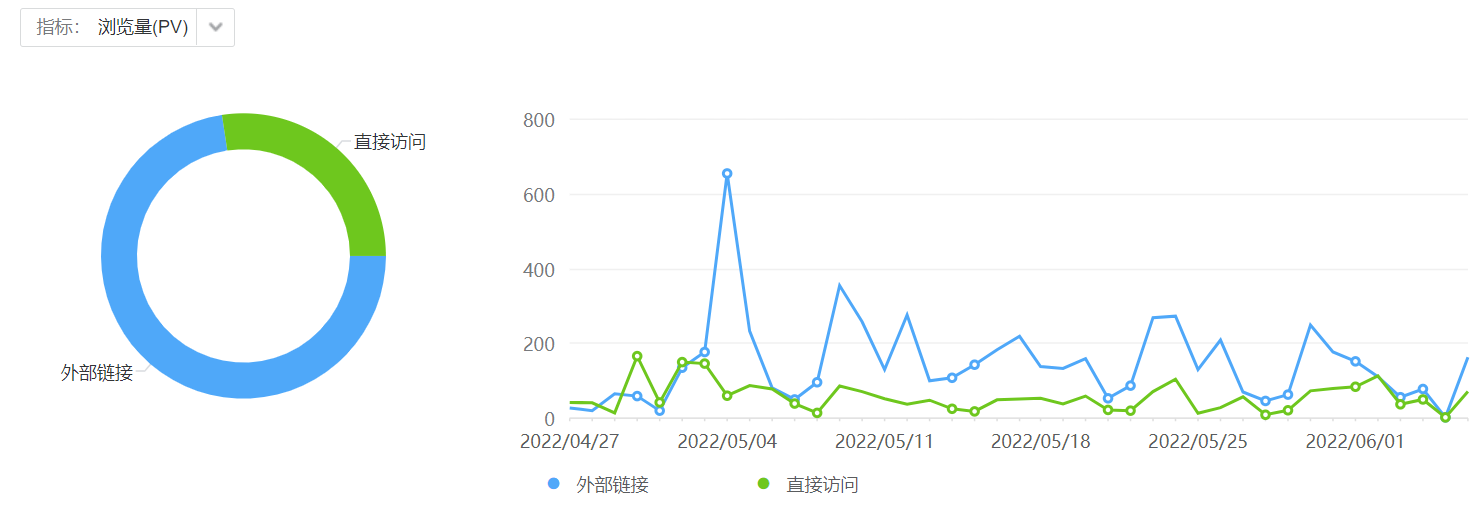
\includegraphics[width=\columnwidth]{figure/0.png}
%   \caption{4 月 27 日至 6 月 7 日的网站浏览量}
%   \label{fig:0}
% \end{figure}
% \begin{figure}[htbp]
%   \centering
%   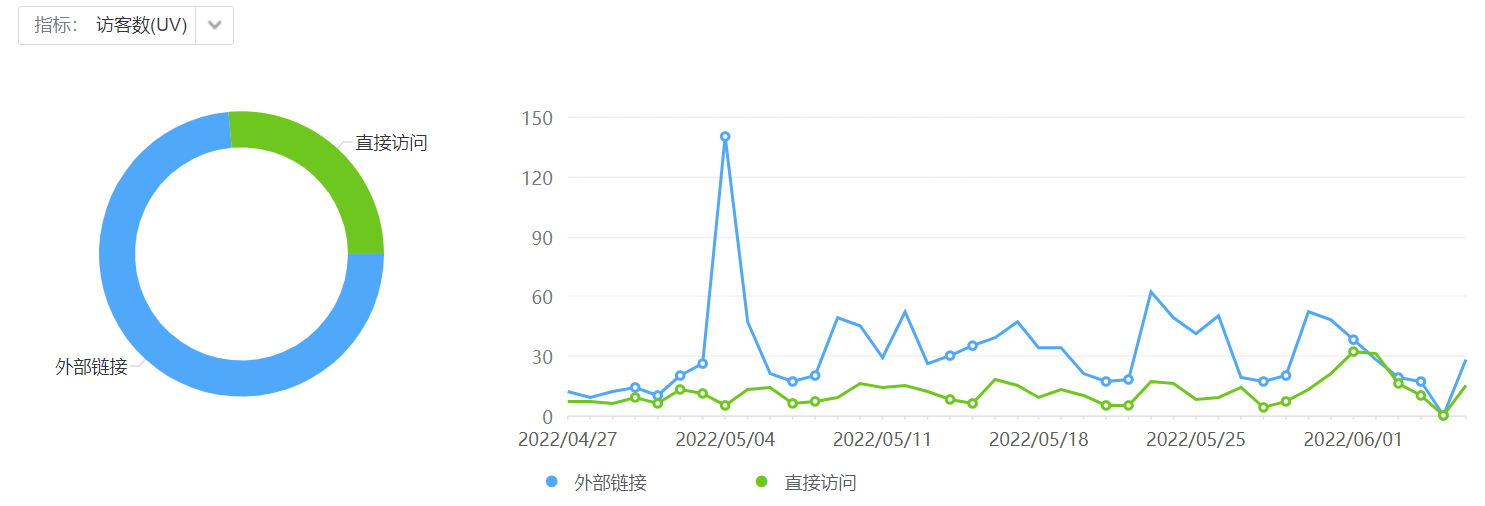
\includegraphics[width=\columnwidth]{figure/1.png}
%   \caption{4 月 27 日至 6 月 7 日的网站访客数}
%   \label{fig:1}
% \end{figure}

工具网站的访问统计如图 \ref{fig:2} 所示,可以看出我们的工具有 1000 名稳定用户。
同时,本工具在 GitHub 上开源,同学们可以进一步完善其功能。

\begin{figure}[htbp]
  \centering
  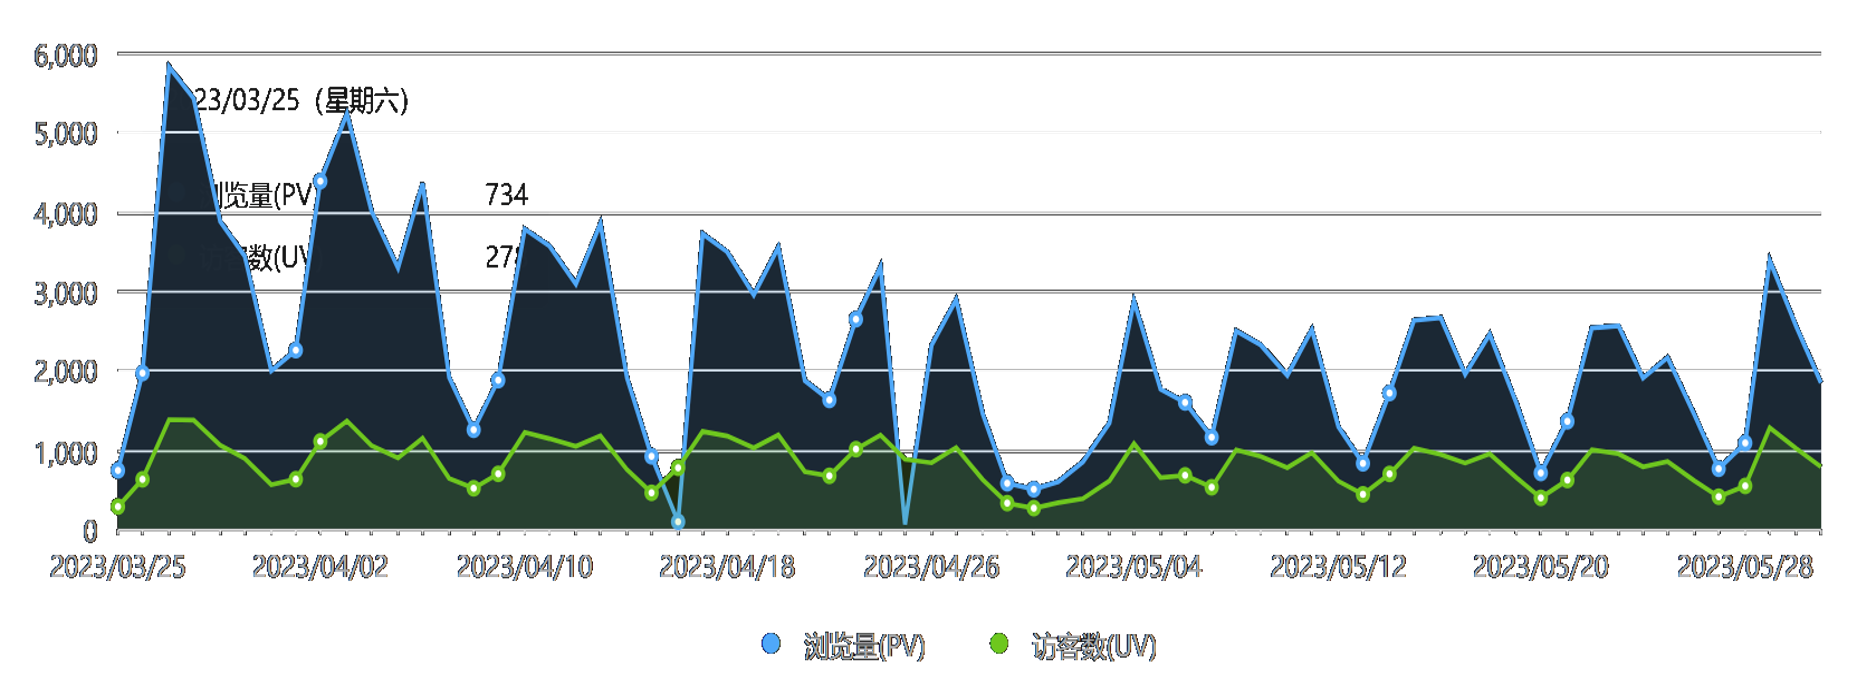
\includegraphics[width=\columnwidth]{figure/2.png}
  \caption{大雾实验工具网站的统计数据}
  \label{fig:2}
\end{figure}

\subsection{蜗壳排课工具}

我们深切理解用户隐私的重要性。因此,排课算法完全在本地通过 JavaScript 运行,任何信息都不会被上传到服务器。用户可以借助 Microsoft Edge 浏览器将本站点作为应用安装,一旦安装完成,即使断网也可以正常使用。

尽管 "蜗壳排课工具" 的推广刚刚开始,但在本学期选课周的日浏览量峰值已经接近 2000,这让我们看到了无限的可能性和光明的前景。

\subsection{我的科大 APP}

我们的产品以其出色的鲁棒性赢得了用户的认可。无论用户进行任何随意的输入,或者尝试进行任何非常规操作,我们的应用都能稳定运行,不会发生崩溃。

尽管 APP 的推广之路充满了挑战,但至今,“我的科大”已经拥有超过 5000 名用户,仅在八月份就新增了超过 1000 名用户。我们每日活跃用户达到 2000 人,每日启动次数约为 2 万次。这些数据充分反映了我们的产品受到了用户的热烈欢迎。